\documentclass[10pt]{article}
\usepackage[letterpaper,landscape,margin=0.65in]{geometry}
\usepackage{graphicx}
\usepackage{booktabs}
\usepackage[T1]{fontenc}
\usepackage{hyperref}
\hypersetup{pdftitle={BINSTD toy-yield citation provenance audit}}
\setlength{\parindent}{0pt}
\setlength{\parskip}{0.45em}
\title{BINSTD toy-yield citation provenance audit}
\author{Validation audit, 22 October 2026}
\date{}
\begin{document}
\maketitle
\vspace{-2em}

\textbf{Question.} Do the two archived BINSTD yield evidence records
have source-bound internal citations, and do their aggregate ratios
agree with the frozen run results?

\textbf{Source chain.} The original $n=17$, $\ell\in\{3,4\}$ panel
found no admissible invariant dimensions and left the yield band
untested. An approved additive amendment moved the panel to
$\ell\in\{8,9\}$. A second approved amendment repeated that panel
under a new Stage-0 seed. Both use 40 targets and the toy exhaustive
$m=3$ factor-base-sum pin.

\begin{center}
\begin{tabular}{lllll}
\toprule
Panel & $\ell$ & $\tau$ hits & open hits & $R_\tau/R_{\rm open}$\\
\midrule
First seed & 8 & 16/40 & 40/40 & 0.4\\
First seed & 9 & 40/40 & 40/40 & 1.0\\
Second seed & 8 & 20/40 & 40/40 & 0.5\\
Second seed & 9 & 40/40 & 40/40 & 1.0\\
\bottomrule
\end{tabular}
\end{center}

\textbf{Verification.} The archived Stage-1 matrix hashes match their
run-result digests. A focused checker recomputes four ratios from the
published aggregate hits and confirms that removing only the 16 new
source-reading notes makes both replacements structurally identical
to their frozen records. On parent commit
\texttt{5e499ba86dfa}, the full ledger validator falls from 136
errors in 38 paths to 120 in 36: exactly 16 citation errors removed,
none added. It still exits 1.

\textbf{Boundary.} All open arms hit 40/40, so the 1.25 ratio cannot be
met at those observed open-arm rates. This audit does not replay
per-target solver work, certify target sampling, or prove empirical
yield in Lean. The first review's preliminary weaken and the
second review's toy-scope rejection are unchanged. No break,
asymptotic or deployed-security conclusion follows.

\newpage
\begin{center}
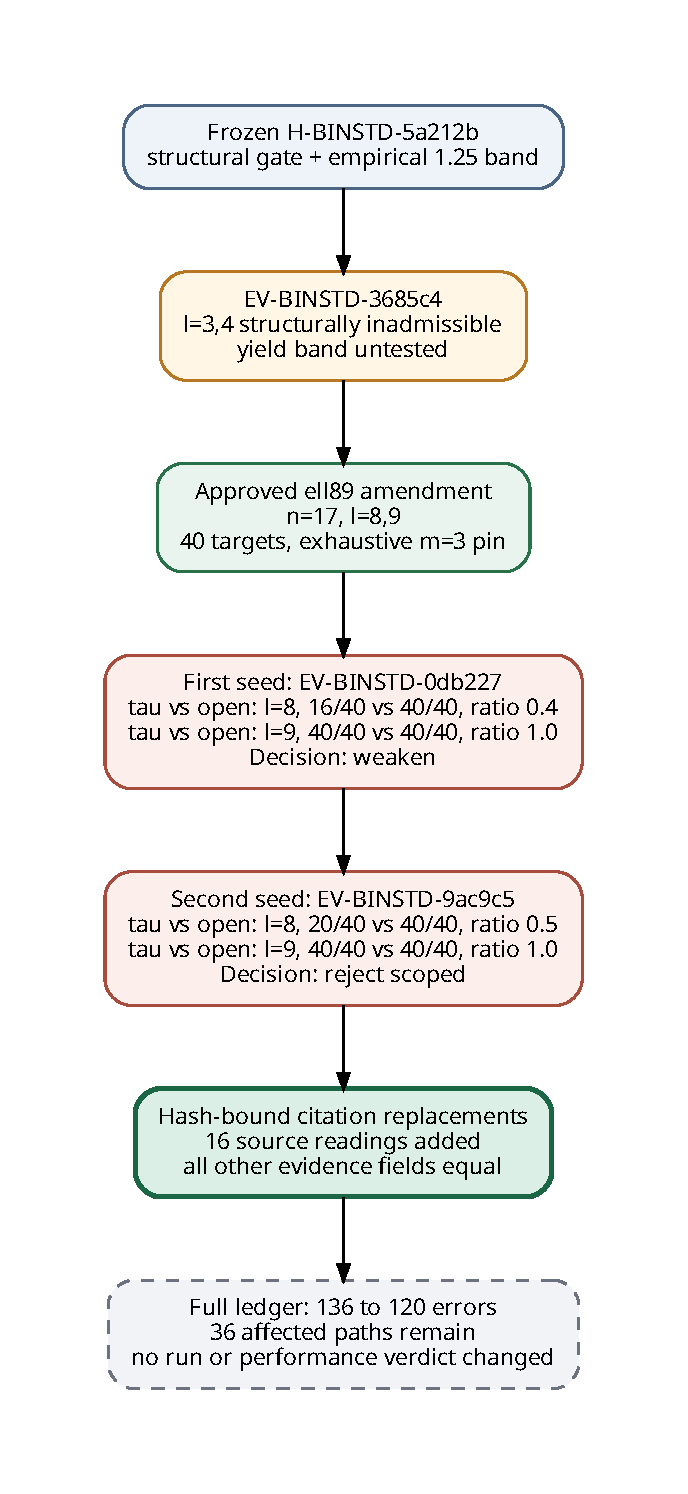
\includegraphics[width=\textwidth,height=0.82\textheight,keepaspectratio]{audit-figure.pdf}
\end{center}
\end{document}
